\begin{figure}[htbp]
\centering
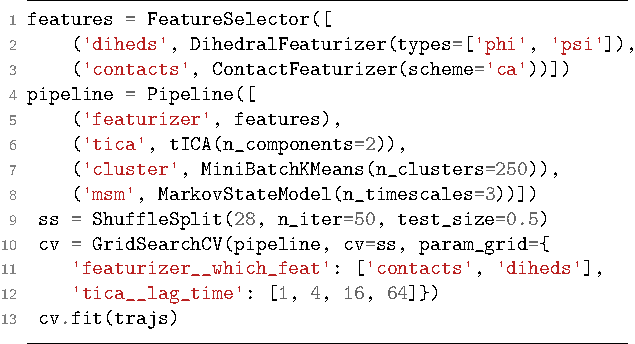
\includegraphics[width=\linewidth]{2-gmrq/code}
\caption{\textbf{Sample GMRQ code.}
    MSMBuilder seamlessly interoperates with the broader Python ecosystem.
    In this code sample, we use \texttt{scikit-learn} for
    algorithm-agnostic data processing and MSMBuilder for
    biophyics-oriented time-series algorithms with the goal of selecting
    model hyperparameters.  Our analysis pipeline is similar to that of
    \cref{sec:example-src} but with a choice of features (between dihedrals
    and contact distances) and tica lag times (among 1, 4, 16, and 64
    steps).  The \texttt{ShuffleSplit} cross-validation scheme runs 50
    iterations of equal partitioning of the 28 trajectories between train and test
    sets, and we perform a full grid-search over parameter choices.  We can
    plot the distribution of scores vs. parameters as in
    \cref{fig:gmrq}.
}
\label{fig:gmrq_code}
\end{figure}

\begin{figure}[htbp]
\centering
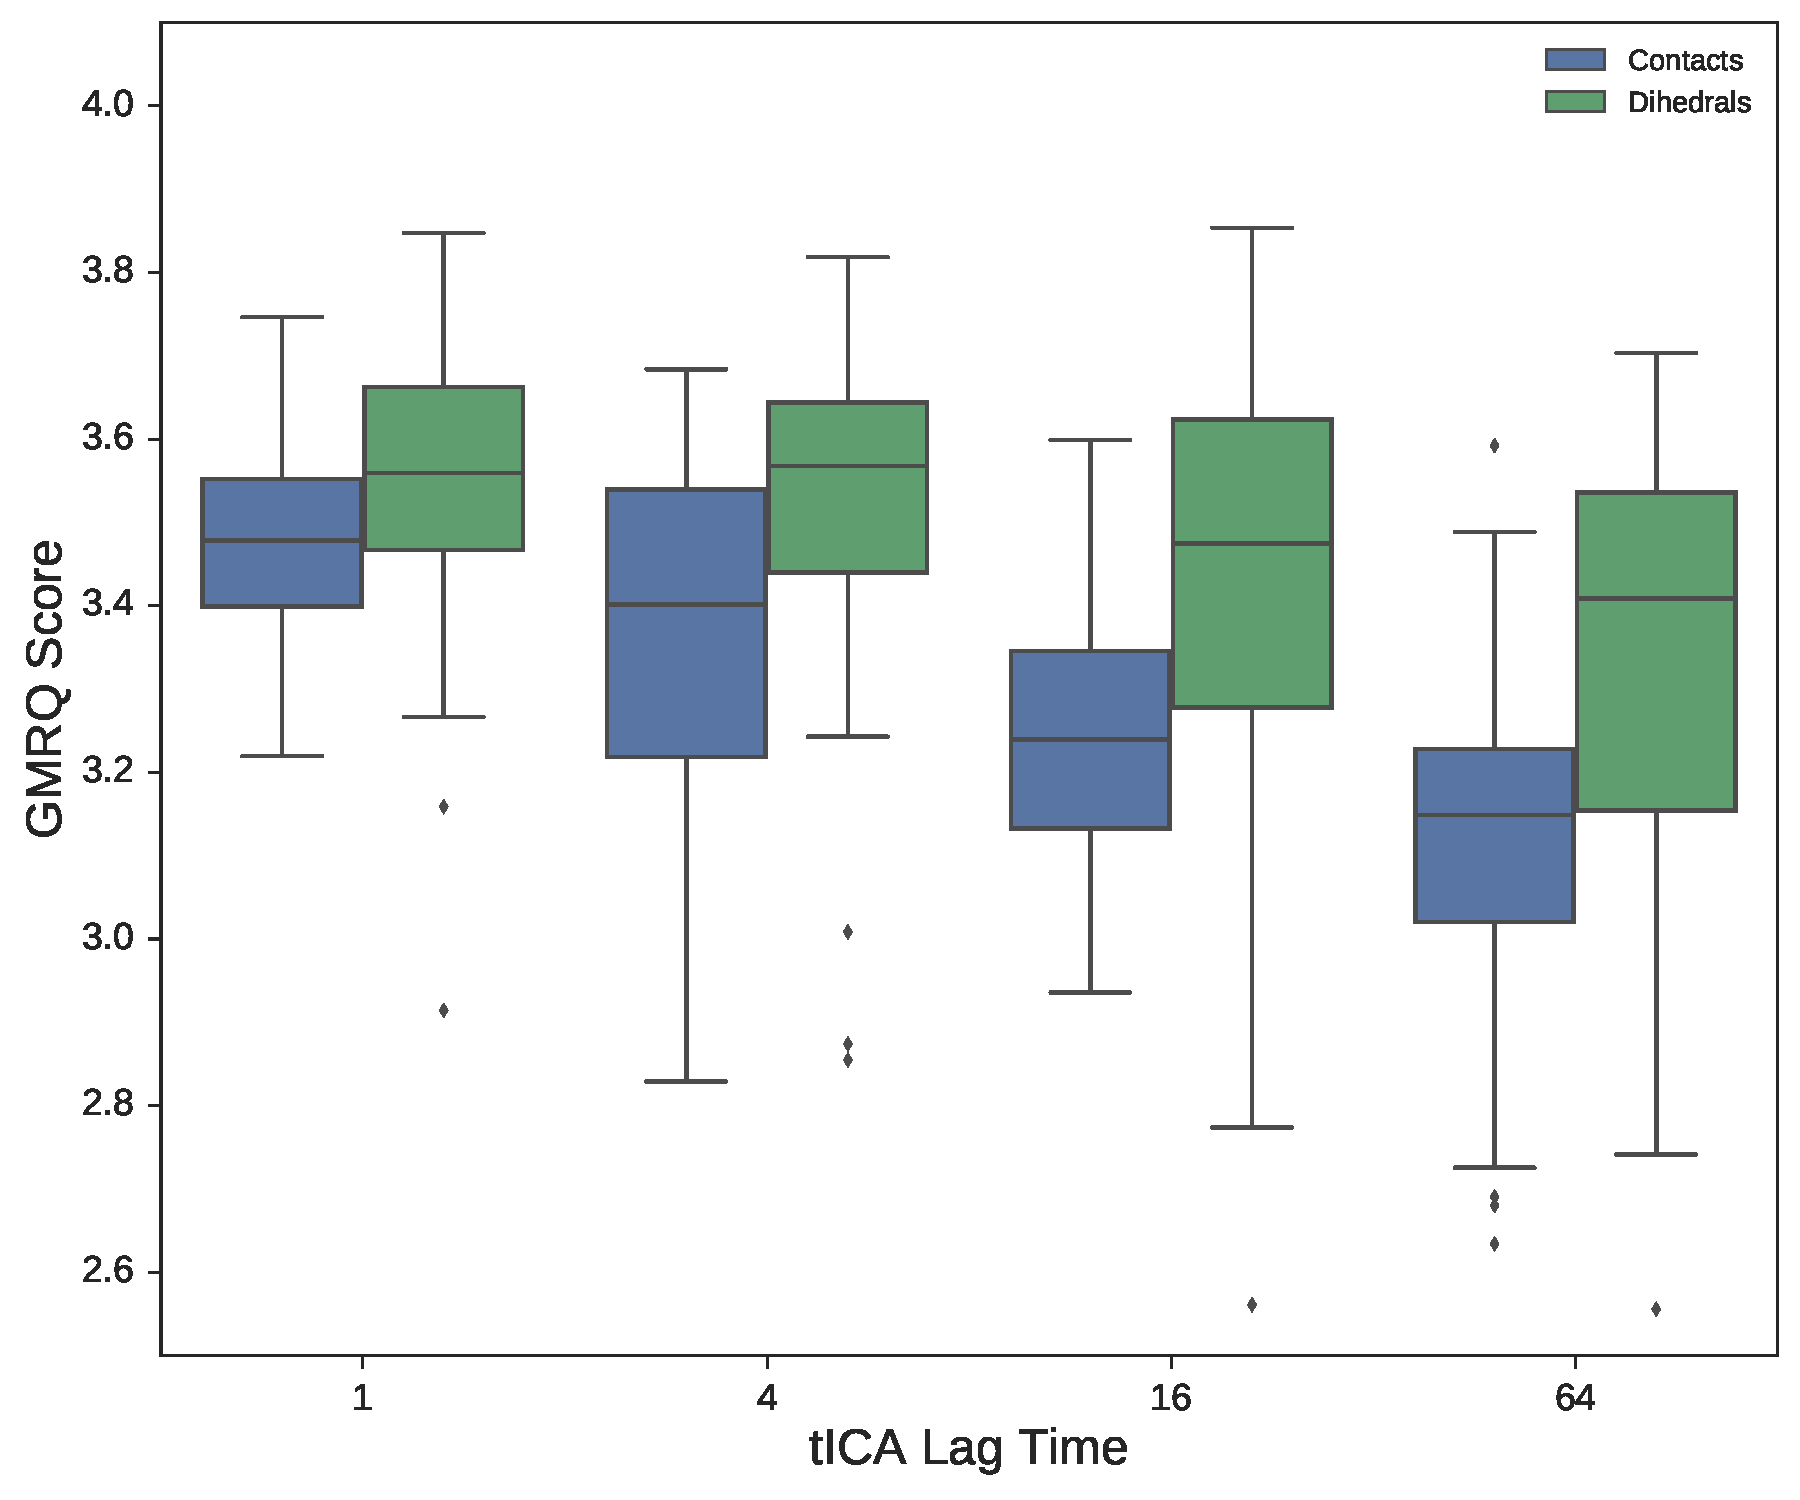
\includegraphics[width=\linewidth]{2-gmrq/plot}
\caption{\textbf{GMRQ parameter selection.}
    MSMBuilder offers robust machinery for selecting hyperparameters that
    cannot \emph{a priori} be learned from the data. Here, we perform
    shuffle-split cross validation over choices of featurization and tICA
    lag time. Historically, these parameters were chosen heuristically.
    With the advent of the GMRQ score and its implementation in MSMBuidler,
    we can choose these parameters in a statistically rigorous way. Here,
    we plot the distribution of scores for each set of of model parameters.
    Note that a higher score is generally an indication of a more predictive
    model. In this example, we find that featurization with dihedral angles
    at a lag time of 4 steps has highest median score and recommend this
    hyperparameter set to be chosen for the final model.
}
\label{fig:gmrq}
\end{figure}

Historically, the heuristic choice of hyperparameters---choices of
protocol---rendered MSM construction as much of an art as a science. It is
clear from \cref{sec:example-src} that there is an abundance of algorithms
available in MSMBuilder. In this instructive example, we use a
scoring functional to select the best models.

\citet{2014-noe-variational} introduced a variational principle that
formalized the definition of a ``good" MSM. In keeping with inspiration
from the broader machine learning community, MSMBuilder extends this
formalism in the context of cross-validation through the work of
\citet{2015-gmrq}. The resulting generalized matrix Rayleigh
quotient (GMRQ) score offers an objective way to pick the best model (i.e. the
appropriate modeling choices) from the given data. Briefly, the GMRQ measures
the ability of a model to capture the slowest dynamics of a system. The
variational principle states that approximating the full phase space
by discrete states  will always yield dynamics that are too fast.
The GMRQ score is a summation of the leading eigenvalues of the model
and therefore provides a measure of ``slow-ness".
A higher score means the model is closer to the variational bound, and
therefore should be prefered over lower scoring models.

In this example, we use the GMRQ score under cross-validation to evaluate
the relative merit of enumerated hyperparameter values when constructing a
model for the Fs peptide \cite{2014-fs-peptide}. The relevant code in
\cref{fig:gmrq_code} sets up a choice between two structural features
(dihedral angles or contact distances) and a choice among tICA lag times.
We perform shuffle-split cross-validation by randomly assigning the 28
trajectories to either the training set or test set. The MSM is learned on
the training set and scored on the test set. By concealing the training
data during scoring, cross-validation guards against overfitting
(overconfidence in excessively complex models). The trajectories are
re-shuffled and this process is repeated to compute an average score for a
given set of hyperparameters.  The scores for each of the 50
cross-validation splits are plotted in a box plot in \cref{fig:gmrq}.
The dihedral angle featurization with a lag-time of 4 steps gives the best model in this
search space.  A simple grid search as performed in this example can become
intractible as the number of hyperparameters (i.e.~the dimension of the
search space) increases. We direct interested users to Osprey
\cite{2016-osprey}, a tool for hyperparameter optimization with a variety
of search strategies and support for parallel computation.
Osprey interoperates with any \texttt{scikit-learn} estimator
including those in MSMBuilder.

This example leverages the \texttt{Pipeline}, \texttt{ShuffleSplit}, and
\texttt{GridSearchCV} machinery from \texttt{scikit-learn}. Additionally,
MSMBuilder uses this library internally for generic machine learning
algorithms such as clustering or PCA. We note that such general algorithms
do not need to be reinvented and re-programmed by the biophysics community.
By delegating some development effort to this widely-used machine learning
library, we ensure that the development of MSMBuilder is focused on
biophysical algorithms and considerations.
This advantage offers rapid adoption of the latest algorithms which have
demonstrated improved ability to build MSMs (e.g. \cite{2015-gmrq}) and a
larger community for code maintenance and longevity.


% vim: tw=75
